\section{Domain Adaptations}
\begin{frame}{Domain Adaptations}
	
			\begin{figure}[!ht]
				\centering
				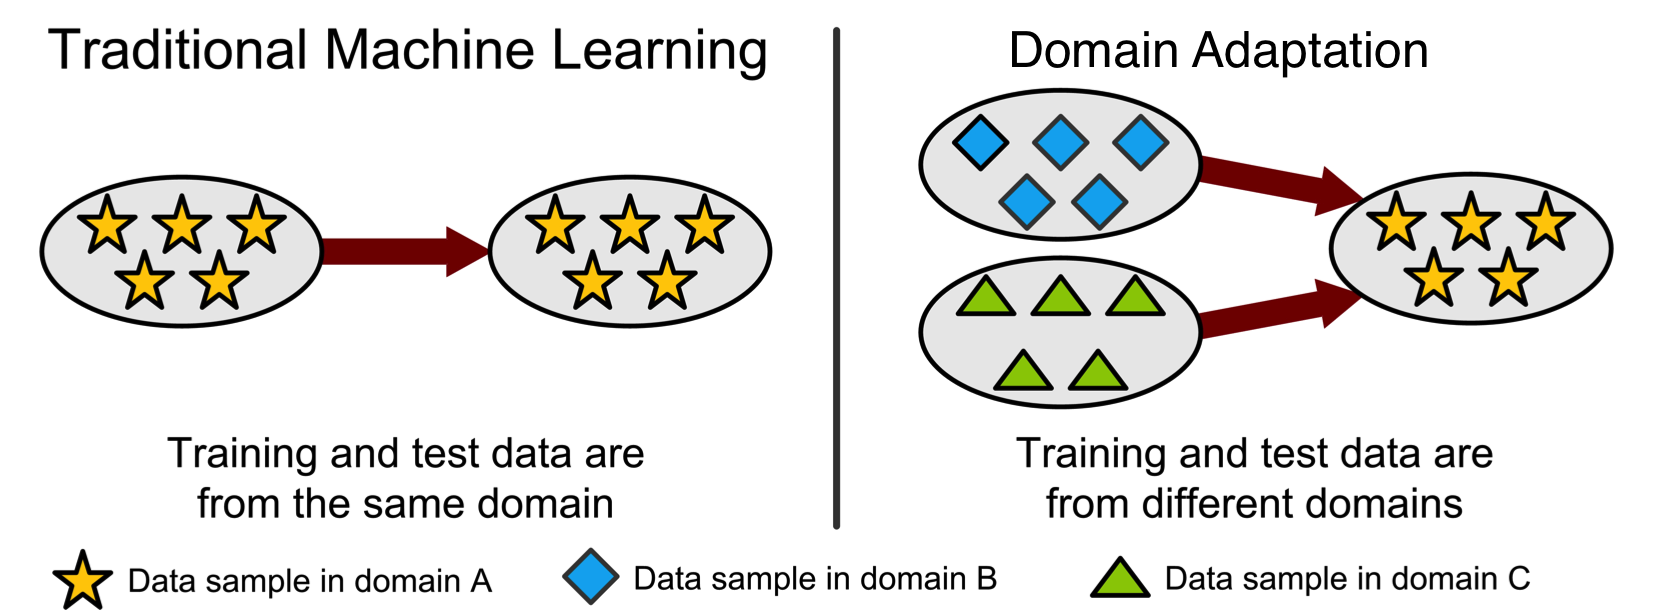
\includegraphics[scale=0.15]{./domainAdaption.png}
			\end{figure}


			\begin{itemize}
				\item Feature Replication \cite{daume2007frustratingly} (FR)
				\item Adaptive Support Vector Machine \cite{yang2007cross} (A-SVM)
				\item Domain Transfer Support Vector Machine \cite{duan2009domain} (DTSVM)
				\item Adaptive Multiple Kernel Learning \cite{duan2012visual} (A-MKL)
			\end{itemize}

\end{frame}






\subsection{Feature Replication}
\begin{frame}{Feature Replication (FR)}
	\begin{itemize}
		\item Mapping functions to augment samples $\{x\}$ from different domains

\begin{equation}\Phi^T(\mathbf{x}) = (\mathbf{x},\mathbf{x},\mathbf{0}), \quad  \Phi^A(\mathbf{x}) = (\mathbf{x},\mathbf{0}, \mathbf{x})\end{equation}

		\item \alert{Kernelized} meaning of the above augmenting\\

			\begin{itemize}
			\item If $x_i$ and $x_j$ come from the same domain, 
\begin{eqnarray}
\hat K(x_i, x_j) &  = & \theta(x_i)^T \cdot \theta(x_j) + \theta(x_i)^T \cdot \theta(x_j) \nonumber \\
 & = & 2 K(x_i, x_j)
\end{eqnarray}

			\item If  $x_i$ and $x_j$ come from different domains,
\begin{eqnarray}
\hat K(x_i, x_j)  & = &  \theta(x_i)^T \cdot \theta(x_j)  \nonumber \\
 & = &  K(x_i, x_j) 
\end{eqnarray}
			\end{itemize}

		\item To summarize,
\[
 \hat K(x_i, x_j) =
  \begin{cases}
   2 K(x_i, x_j) & \text{if } x_i \text{ and } x_j \text{ come from the same domain}\\
   K(x_i, x_j)   & \text{otherwise} 
  \end{cases}
\]		
	\end{itemize}
\end{frame}

\subsection{Adaptive SVM}
\begin{frame}{Adaptive Support Vector Machine (A-SVM)}


\begin{tikzpicture} [scale = 0.88] 
% Auxiliary Domain
\node[circle, fill = gray!30] (one) at (0, 0) {$D^A_1$};
\node[circle, fill = gray!30] (two) at +(-90: 1.5) {$D^A_2$};

\draw[fill=black] +(-90:2.3) circle (0.05);
\draw[fill=black] +(-90:2.8) circle (0.05);
\draw[fill=black] +(-90:3.3) circle (0.05);

\node[circle, fill = gray!30] (three) at +(-90: 4) {$D^A_M$};


\node[rectangle, fill = gray!30] (cone) at (0: 2) {$f_1^A(\mathbf{x})$};
\node[rectangle, fill = gray!30] (ctwo) at (2, -1.5) {$f_2^A(\mathbf{x})$};

\draw[fill=black] +(2, -2.3) circle (0.05);
\draw[fill=black] +(2, -2.8) circle (0.05);
\draw[fill=black] +(2, -3.3) circle (0.05);

\node[rectangle, fill = gray!30] (cthree) at (2,-4) {$f_M^A(\mathbf{x})$};


\node[draw] (plus) at (5.4, -2) {$+$};

% Add edges
\draw[->, line width = 2pt] (one) -- (cone);
\draw[->, line width = 2pt] (two) -- (ctwo);
\draw[->, line width = 2pt] (three) -- (cthree);

\draw[->, line width = 2pt] (cone) -- (plus) node[pos= 0.5, sloped, above]{$t_1$};
\draw[->, line width = 2pt] (ctwo) -- (plus) node[pos= 0.5, sloped, above]{$t_2$};
\draw[->, line width = 2pt] (cthree) -- (plus) node[pos= 0.5, sloped, above]{$t_M$};

\draw[black,thick,dotted] ($(one.north west)+(-0.3,0.6)$)  rectangle ($(plus.south east)+(0.3,-2.6)$);

\node (auxiliary) at ( 4.4, 0.4) {Auxiliary Domain};

% Target Domain
\node[circle, fill = gray!30] (t) at (0, -5.8) {$D^T_l$};
\node[rectangle, fill = gray!30] (tF) at (3, -5.8) {$\Delta f(\mathbf{x}) = w^T \phi(x)$};
\node[draw](plus2) at (6.7,-2.9) {$+$};

\draw[->, line width = 2pt] (t) -- (tF);
\draw[->, line width = 2pt] (plus) -- (plus2);
\draw[->, line width = 2pt] (tF) .. controls +(right: 3) .. (plus2);

\draw[black,thick,dotted] ($(t.north west)+(-0.3,0.2)$) rectangle ($(tF.south east)+(0.3,-1)$);

\node (target) at (2, -6.7) {Target Domain};

% Decision Function
\node[rectangle] (df) at (8.2, -2.9) {$f(\mathbf{x})=$};

\node[fill = blue!30](partOne) at (10.2, -2.9) {$\sum_{k=1}^M t_k f_{k}^A(\mathbf{x})$};
\node[fill= red!30](partTwo) at (12.6, -2.9) {$ \Delta f(\mathbf{x})$};
\node at (11.8, -2.9) {$+$};

\draw[->, line width = 2pt] (plus2) -- (df);


% Two key points of decision function
\node (keyOne) at (10.2, -1.5) {separates the labeled examples in $D^T_l$ well};

\node (keyTwo) at (9.7, -5) {seeks a hyperplane which is close to};
\node (keyThree) at (9.8, -5.5) {the boundaries of auxiliary classifiers.};

\draw[->, line width = 2pt] (keyOne) -- (partTwo);
\draw[->, line width = 2pt] (keyTwo) -- (partOne);

\end{tikzpicture}.
\end{frame}


\subsection{Domain Transfer SVM}
\begin{frame}{Domain Transfer Support Vector Machine (DTSVM)}
	\begin{itemize}
		\item Some way to reduce the difference in distribution of $D^T$ and $D^A$
		\begin{center}
		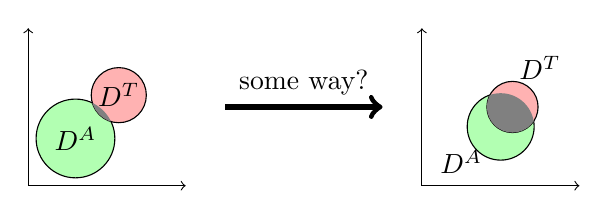
\begin{tikzpicture} [scale = 0.5]
		    \draw [->] (0,0) -- (4,0);
		    \draw [->] (0,0) -- (0,4);
		    
			\draw[fill=green!30] (1.2,1.2) circle (1) node {$D^A$};
			\draw[fill=red!30] (2.3,2.3) circle (0.7) node {$D^T$};

		    \begin{scope}
		    \clip (1.2,1.2) circle (1);
		    \fill [color = gray] (2.3,2.3) circle (0.7);
		    \end{scope}

		    \draw [->] (10,0) -- (14,0);
		    \draw [->] (10,0) -- (10,4);


		    \draw[fill=green!30] (12,1.5) circle (0.85);
			\draw[fill=red!30] (12.3,2) circle (0.65);		   

		    \begin{scope}
		    \clip (12,1.5) circle (0.85);
		    \fill [color = gray] (12.3,2) circle (0.65);
		    \end{scope}

		    \node () at (11,0.6) {$D^A$};
		    \node () at (13, 3) {$D^T$};

		    \draw[->, line width = 2pt] (5,2) -- (9,2) node[pos=0.5, above] {some way?};
		\end{tikzpicture}
		\end{center}

		\item Seek a special kernel function \alert{$\varphi(x)$} which minimizes the difference 
			\begin{itemize}
				\item Find the optimal weights \alert{($d_1, d_2, ..., d_M$)} of multiple kernels

		\begin{center}
		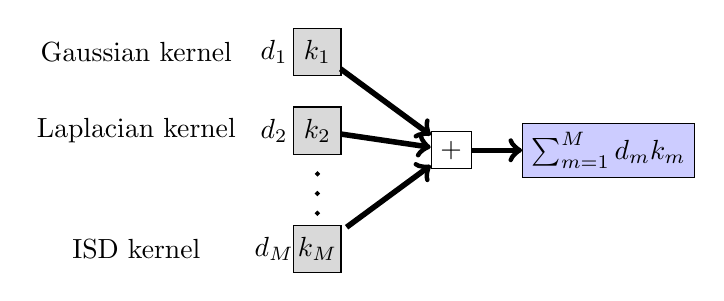
\begin{tikzpicture} [scale = 0.5]
		\draw[fill = gray!30] (0, 0) rectangle (1.2,1.2) node[pos = 0.5] (dm) {$k_M$};
		\node at (-0.5, 0.6) {$d_M$};
		\node at (-4, 0.6) {ISD kernel};


		\draw[fill=black] (0.6, 1.5) circle (0.05);
		\draw[fill=black] (0.6, 2) circle (0.05);
		\draw[fill=black] (0.6, 2.5) circle (0.05);

		\draw[fill = gray!30] (0, 3) rectangle (1.2,4.2) node[pos = 0.5] (d2) {$k_2$};
		\node at (-0.5, 3.6) {$d_2$};
		\node at (-4, 3.6) {Laplacian kernel};


		\draw[fill = gray!30] (0, 5) rectangle (1.2, 6.2) node[pos = 0.5] (d1) {$k_1$};
		\node at (-0.5, 5.6) {$d_1$};
		\node at (-4, 5.6) {Gaussian kernel};

		\node[draw] (plusOne) at (4, 3.1) {$+$};

		\node[draw, fill = blue!20] (sumOne) at (8, 3.1) {$\sum_{m=1}^{M} d_m k_m$};

		% edges
		\draw[->, line width = 2pt] (d1) -- (plusOne);
		\draw[->, line width = 2pt] (d2) -- (plusOne);
		\draw[->, line width = 2pt] (dm) -- (plusOne);
		\draw[->, line width = 2pt] (plusOne) -- (sumOne);


		\end{tikzpicture} 
		\end{center}


			\end{itemize}

	\end{itemize}
\end{frame}

\begin{frame}
	\begin{itemize}
		\item Define the mismatch between $D^A$ and $D^T$ as 
\begin{equation}
DIST_k(\mathcal{D}^A, \mathcal{D}^T) = \norm{\frac{1}{n_A} \sum_{i=1}^{n_A} \varphi(x_i^A) - \frac{1}{n_T} \sum_{i=1}^{n_T} \varphi (x_i^T)}
\end{equation}

		\item Simplify the square of equation (4) to
\begin{equation}
DIST_k^2(\mathcal{D}^A, \mathcal{D}^T) = \text{tr}(\mathbf{KS})
\end{equation}

where $\mathbf{s} = [\underbrace{\frac{1}{n_A}, ..., \frac{1}{n_A}}_\text{$n_A$}, \underbrace{\frac{-1}{n_T},...,\frac{-1}{n_T}}_\text{$n_T$}] ^T$, $\mathbf{S = s s^T }$, $\mathbf{K = \begin{bmatrix} K^{A,A} & K^{A,T} \\ K^{T, A} & K^{T,T}\\  \end{bmatrix}}$

	\item Incorporate \alert{$\mathbf{d} = [d_1, d_2, ..., d_M]^T$} into equation (5)
\begin{equation}
DIST_k^2(\mathcal{D}^A, \mathcal{D}^T) = \Omega(\mathbf{d}) = \mathbf{h^T d}
\end{equation}

where $\mathbf{h} = [tr(\mathbf{K_1 S}), \cdots, tr(\mathbf{K_MS})]^T$, and $\mathbf{K_m} = [\varphi(x)^T \varphi(x)]$ is the $m$th base kernel matrix 

	\end{itemize}
\end{frame}

\begin{frame}
	\begin{itemize}
		\item Optimization problem of DTSVM: 
			\begin{enumerate}
			    \item Distribution mismatch \tikz[na] \node[coordinate] (n1) {};
				\item SVM structural risk function \tikz[na] \node[coordinate] (n2) {};
			\end{enumerate}

			\begin{equation}
			\text{minimize} \quad G(\mathbf{d}) = 
			\tikz[baseline]{\node[fill=green!20,anchor=base] (t1)
			{$\frac{1}{2} \Omega^2(\mathbf{d})$};}
			+ \theta 
			\tikz[baseline]{\node[fill=red!20,anchor=base] (t2)
			{$J(\mathbf{d})$};}
			\end{equation} 

			where 
			\resizebox{.8 \textwidth}{!}{ 
			  $J(\mathbf{d}) = \underset{\boldsymbol{\alpha}}{\max} \; \sum_i \alpha_i - \frac{1}{2} \sum_{i,j} y_i y_j \alpha_i \alpha_j  (\sum_{m=1}^M d_m \; \varphi_m (x_i) ^T \varphi_m (x_j))$ 
			}


			\begin{tikzpicture}[overlay]
				\path[->, green, thick] (n1) edge [bend left] (t1); 
				\path[->, red!20, thick] (n2) edge [bend left] (t2); 
			\end{tikzpicture}

		\item Iteratively update coefficient $\mathbf{d}$ and the dual variable $\boldsymbol{\alpha}$

			\begin{enumerate}
				\item Update the dual variable $\boldsymbol{\alpha}$\\
				\item Update the coefficient $\mathbf{d}$ using \alert{gradient descent method} \\
				\begin{equation}
				\mathbf{d}_{t+1} = (1 - \eta_t) \mathbf{d}_{t} + \eta_t \mathbf{d}_t^{new}
				\end{equation}

				where 
				\resizebox{.76 \textwidth}{!}{ 		
				$\mathbf{d}_t^{new} = \theta(\mathbf{h h^T} + \varepsilon \mathbf{I_M})^{-1} \mathbf{q}$, 

				$\mathbf{q} = [\frac{1}{2}(\boldsymbol{\alpha}_t \diamond \mathbf{y})^T \mathbf{K}_1 (\boldsymbol{\alpha}_t \diamond \mathbf{y}), \cdots, \frac{1}{2}(\boldsymbol{\alpha}_t \diamond \mathbf{y})^T \mathbf{K}_M (\boldsymbol{\alpha}_t \diamond \mathbf{y})]$},

				$\eta_t$ is the learning rate.
			\end{enumerate}

		\item Final decision function
		\begin{equation}
		f(x) = \sum_{i=1}^{n} {\alpha}_i y_i \bigg(\sum_{m=1}^{M} d_m \mathbf{K}_m(x_i, x) \bigg) + b
		\end{equation}

	\end{itemize}
\end{frame}

\subsection{Adaptive MKL}
\begin{frame}{Adaptive Multiple Kernel Learning \cite{duan2012visual} (A-MKL)}
	\begin{itemize}

		\item Adaptive SVM
			\begin{equation}
			f(x) = 
			\tikz[baseline]{\node[fill=green!20,anchor=base] (t1)
			{$\sum_{k=1}^M t_k f_{k}^A(x)$};} 
			+ \Delta f(x)
			\end{equation}

		\item Domain Transfer SVM
			\begin{equation}
			f(x) = 
			\tikz[baseline]{\node[fill=red!20,anchor=base] (t2)
			{$\sum_{m=1}^{M} d_m w_m^T \varphi_m(x)$};} + b 
			\end{equation}

		\item Adaptive MKL
			\begin{equation}
			f(x) = 
			\tikz[baseline]{\node[fill=green!20,anchor=base] (n1)
			{$\sum_{p=1}^{P} \beta_p f_p(x)$};}
			+ 
			\tikz[baseline]{\node[fill=red!20,anchor=base] (n2)
			{$\sum_{m=1}^{M} d_m w_m^T \varphi_m(x)$};} + b 
			\end{equation}

		\begin{tikzpicture}[overlay]
			\path[->, green, thick] (t1) edge [bend right] (n1); 
			\path[->, red, thick] (t2) edge [bend left] (n2); 
		\end{tikzpicture}

			\begin{itemize}
				\item Seek a hyperplane which is close to that of all labeled samples
				\item Reduce the mismatch of different domains
			\end{itemize}

	\end{itemize}

\end{frame}

\subsection{Experiments}
\begin{frame}{Experiments of Domain Adaptation Approaches}

\begin{itemize}

	\item Data set
	
  \begin{table}[!ht]
    \begin{center}
      \scalebox{0.7}{
      \begin{tabular}{cccccccc}
      \hline
      \head{} & \head{Wedding} & \head{Sports} & \head{Show} & \head{Picnic} & \head{Parade} & \head{Birthday} & \head{Total}\\
      \hline
      Kodak & 27 & 75 & 57 & 6 & 14 & 16 & 195\\
      Youtube & 91 & 260 & 200 & 85 & 119 & 151 & 906\\
      \hline
      \end{tabular}
    }
    \end{center}
    \caption{Number of videos in each class from Kodak and Youtube}
  \end{table}

  \item Distances using various approaches

	\begin{table}[!ht]
	  \begin{center}
	  \scalebox{0.7}{
	    \begin{tabular} {cl}
	    \hline
	    \head{Setting Name} & \head{Content}\\
	    \hline
	    MAP(1) & Level 0 distance in Aligned Space-Time Pyramid Matching \\
	    MAP(2) & \alert{unaligned} Level 1 distance in Aligned Space-Time Pyramid Matching\\
	    MAP(3) & \alert{aligned} Level 1 distance in Aligned Space-Time Pyramid Matching \\

	    MAP(4) & Level 0 distance using histograms built in \alert{``tfc''} weighting scheme \\

	    MAP(5) & Level 0 distance using histograms built by \alert{straightforward soft assignment} \\
	    MAP(6) & Level 0 distance using histograms built by \alert{GMM soft assignment} \\

	    MAP(7) & \vtop{\hbox{\strut distances calculated by \alert{specialized GMMs} built on 128 dimensional SIFT} \hbox{\strut features with spherical covariance}} \\

	    MAP(8) & \alert{two} set of distances: MAP(3) + MAP(6) \\
	    \hline
	    \end{tabular}
	  }
	    \end{center}
	    \caption{Experimental distance set}
	\end{table}

\end{itemize}
\end{frame}

\begin{frame}
	\begin{itemize}
		\item Base kernel matrices
			\begin{columns}
				\column{0.33\textwidth}
					\begin{table}[!ht]
					    \begin{center}
					      \scalebox{0.75}{
					      \begin{tabular}{cc}
					      \hline
					      \head{Kernel type} & \head{Kernel function}\\
					      \hline
					      Gaussian & $\exp(-\gamma D^2(I_i, I_j)$ \\
					      Laplacian & $\exp(- \sqrt{\gamma} D(I_i, I_j)$ \\
					      ISD & $\frac{1}{\gamma D^2(I_i, I_j) + 1}$ \\
					      ID & $\frac{1}{\sqrt{\gamma}D(I_i, I_j) + 1}$\\
					      \hline
					      \end{tabular}
					      }
					    \end{center}
					\end{table}

				\column{0.67\textwidth}
					\begin{itemize}
						\item $D(I_i, I_j)$ represents the distance between $I_i$ and $I_j$

						\item $\gamma = 2^l \gamma_0$
							\begin{itemize}
								\item $\gamma_0 = \frac{1}{A}$, $A$ is the mean value of the squared distances between training samples

								\item $l \in \alert{(-3, -2,\cdots, 1)}$
							\end{itemize}
						
						\item \alert{$4 \times 5$} combinations $\rightarrow$ 20 base kernel matrices
					\end{itemize}
			\end{columns}

		\item Division of training and testing samples
			\begin{itemize}
				\item 3 videos for each class in Kodak domain as $\mathcal{D}_l^T$, and the left 

				\item the left Kodak videos as $\mathcal{D}_u^T$

				\item all Youtube videos as fully labeled $\mathcal{D}^A$ 
			\end{itemize}

		\item Evaluation metric: Mean Average Precision
			
			% \begin{equation}
			% \resizebox{.25\hsize}{!}{
			% $AP = \frac{1}{R} \sum_{j} \frac{R_j}{j} \times I_j$}
			% \end{equation} 

			% \begin{itemize}
			% 	\item $R_j$ be the number of true relevant videos in the top $j$ list

			% 	\item $I_j = 1$ if and only if the $j$th video is true relevant, otherwise $I_j = 0$ 
			% \end{itemize}
	\end{itemize}	
\end{frame}

\begin{frame}{Experimental Results}
	\begin{table}[!ht]
  \begin{center}
  \scalebox{0.7}{

    \begin{tabular} {ccccccc}
    \hline
    \head{} &\head{    \tikz[baseline]{\node[anchor=base] (one1) {SVM\textunderscore T};}              } &\head{SVM\textunderscore AT} &\head{FR} &\head{A-SVM}  &\head{DTSVM} &\head{A-MKL} \\
    \hline
    MAP(1) & $44.33 \pm 2.61$ & $52.21 \pm2.54$ & $52.33 \pm 2.20$ & $47.03 \pm3.26$ & $47.14 \pm3.26$ & $54.29 \pm 2.21$ \\

    MAP(2) & $43.55 \pm3.46$&  $55.37 \pm2.26$&  $55.95 \pm 3.79$  &$45.86 \pm4.39$  &$50.97 \pm 1.38$ & $54.26 \pm 3.46$ \\

    MAP(3) & $44.08 \pm 3.25$ & $57.56 \pm3.02$ & $53.91 \pm 1.48$ & $45.42 \pm 3.62$  & $53.32 \pm 2.56$ & $\mathbf{57.45 \pm 1.64}$ \\

    MAP(4) &
    $ 45.27 \pm 1.63$ & $ 51.83 \pm 2.27$ & $52.55 \pm 2.00$ & $45.94 \pm 1.70 $  & $52.31  \pm 2.56$ & $53.05\pm 2.21$ \\

    MAP(5) & 
    $44.79 \pm 2.55$ & $47.80 \pm 1.67$ & $51.89 \pm 1.99$ & $47.41 \pm 3.13$ & $45.05 \pm 4.07$ & $51.08 \pm 2.87$ \\

    \tikz[baseline]{\node[anchor=base] (two1) {MAP(6)};} & $45.20 \pm 3.04$ & $56.90 \pm 2.79$ & $54.03\pm 4.02$ & $46.62 \pm 3.14 $ & $53.41 \pm 3.29$ & \tikz[baseline]{\node[anchor=base] (two2) {$\mathbf{59.16 \pm 3.38}$};} \\

    MAP(7) &
    $32.91 \pm 2.20$ & $33.15 \pm 1.78$ & $41.78 \pm 3.98 $ &$37.07 \pm 3.52$& $\mathbf{46.61 \pm 2.41}$ & $35.88 \pm 1.98$ \\

    MAP(8) & $ 44.69\pm 2.84$ &   \tikz[baseline]{\node[anchor=base] (one2) {$ 60.21 \pm 1.94 $};} & $55.29 \pm 3.00$ & $46.28 \pm 4.23 $  & $ 57.01 \pm 2.45 $ & \alert{$\mathbf{61.40 \pm 1.91}$} \\

    \hline
    \end{tabular}
    }

    \end{center}
    \caption{Means and standard deviations (percent) of MAPs over six events}
\end{table}



		\begin{enumerate}
		 	\item  In all cases, \tikz[baseline, inner sep=0] \node[anchor=base] (one3) {SVM\_AT}; performed better than SVM\_T 
		 	\item \tikz[na] \node[coordinate] (two3) {two3};  Gaussian soft assignment outperformed the other approaches

		 	\item DTSVM performed amazingly in MAP(7)
		 	\item A-MKL performed the best by selecting two distance matrices smartly
		 	
		\end{enumerate}

		\begin{tikzpicture}[overlay]
			% first item
			 \draw[red!40,thick,line width = 2] ($(one1.north west)+(-1,-0.5)$)  rectangle ($(one2.south east)+(-2,0.5)$) ;
			 \draw [->, line width = 2, red!40] ($(one2.south east)+(-3,0.4)$) -- (one3);

			 % second item
			 \draw[green!40,thick,line width = 2] ($(two1.north west)+(-0.2,0.1)$)  rectangle ($(two2.south east)+(-1,0.35)$) ;
			 \path[green, line width = 2, green!40, ->] ($(two1.south west)+(-0.2,0.5)$) edge [out = -100, in = 180] (two3);

		\end{tikzpicture}

\end{frame}

\begin{frame} {Recognition Accuracy as Evaluation Metric}
	\begin{itemize}
		\item Recognition accuracy is defined as 
			\begin{equation}
			\text{recognition accuracy} = \frac{\text{correct predictions}}{\text{number of testing samples}}
			\end{equation}
		\item SVM multi-class classification


			\begin{columns}
				\column{0.4\textwidth}
					\begin{center}
					one-vs-all
					\end{center}
					\vspace{3 mm}
					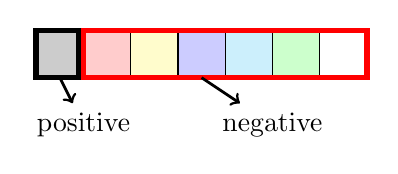
\begin{tikzpicture} [scale=0.3]

						\draw[fill=black!20] (0,0) rectangle (2, 2);
						\draw[fill=red!20] (2,0) rectangle (4, 2);
						\draw[fill=yellow!20] (4,0) rectangle (6, 2);
						\draw[fill=blue!20] (6,0) rectangle (8, 2);
						\draw[fill=cyan!20] (8,0) rectangle (10, 2);
						\draw[fill=green!20] (10,0) rectangle (12, 2);


						\draw[line width = 2pt, black] (0,0) rectangle (1.8, 2);
						\draw[line width = 2pt, red] (2,0) rectangle (14, 2);

						\coordinate (A1) at (1,0);
						\coordinate (B1) at (7,0);

						\node (A2) at (2, -2) {positive};
						\node (B2) at (10, -2) {negative};

						\draw[->, line width = 1pt] (A1) -- (A2);
						\draw[->, line width = 1pt] (B1) -- (B2);

					\end{tikzpicture}

					$n$ classes $\rightarrow$ $n$ classifiers 


				\column{0.4\textwidth}
					\begin{center}
					one-vs-one
					\end{center}

					\vspace{3 mm}
					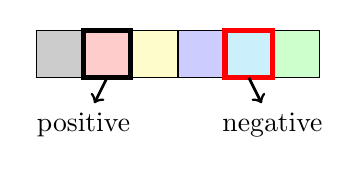
\begin{tikzpicture} [scale=0.3]

						\draw[fill=black!20] (0,0) rectangle (2, 2);
						\draw[fill=red!20] (2,0) rectangle (4, 2);
						\draw[fill=yellow!20] (4,0) rectangle (6, 2);
						\draw[fill=blue!20] (6,0) rectangle (8, 2);
						\draw[fill=cyan!20] (8,0) rectangle (10, 2);
						\draw[fill=green!20] (10,0) rectangle (12, 2);


						\draw[line width = 2pt, black] (2,0) rectangle (4, 2);
						\draw[line width = 2pt, red] (8,0) rectangle (10, 2);

						\coordinate (A1) at (3,0);
						\coordinate (B1) at (9,0);

						\node (A2) at (2, -2) {positive};
						\node (B2) at (10, -2) {negative};

						\draw[->, line width = 1pt] (A1) -- (A2);
						\draw[->, line width = 1pt] (B1) -- (B2);

					\end{tikzpicture}
					$n$ classes $\rightarrow$ $\frac{n(n-1)}{2}$ classifiers 
			\end{columns}

			




	\end{itemize}

\end{frame}

\begin{frame}
		\begin{table}[!ht]
	  	\centering
	  	\scalebox{0.6}{
	    \begin{tabular} {cccccccc}
	    \hline
	    \head{} &\head{SVM\textunderscore T} &\head{SVM\textunderscore AT} &\head{FR} &\head{A-SVM}  &\head{DTSVM} &\head{A-MKL} \\
	    \hline
	    one-vs-all & $49.94 \pm 6.96 $ & $ 57.85\pm 1.91$ & $57.18\pm8.59$ & $ 48.25\pm8.43$  & $ 55.82\pm0.83$ & $ \mathbf{58.87 \pm 0.90}$ \\
	    
	    one-vs-one & $ 33.67\pm 14.67$ & $ 51.64\pm 0.45 $ & $57.18 \pm 6.21$ & $36.05 \pm 12.62$ & $50.85\pm0.80$ & $ 55.14\pm 2.10$ \\
	    \hline
	    \end{tabular}
	    }

	    \caption{Means and standard deviations (percent) of average recognition accuracies}
		\end{table}

		\begin{table}[!ht]
			\centering
		  \scalebox{0.6}{
		    \begin{tabular} {cccccccc}
		    \hline
		    \head{} &\head{SVM\textunderscore T} &\head{SVM\textunderscore AT} &\head{FR} &\head{A-SVM} &\head{DTSVM} &\head{A-MKL} \\
		    \hline
		    one-vs-all & $0.98$ & $8.54$ & $10.53$ & $12.52$ & $11.33$ & $27.87$ \\
		    
		    one-vs-one & $1.49$ & $4.08$ & $5.68$ & $7.16$ & $5.05$ & $10.94$\\
		    \hline
		    \end{tabular}
		    }

		    \caption{Average running time (seconds)}
		\end{table}

		\begin{columns}
			\column{0.5\textwidth}
					\begin{figure}[!ht]
						\centering
						  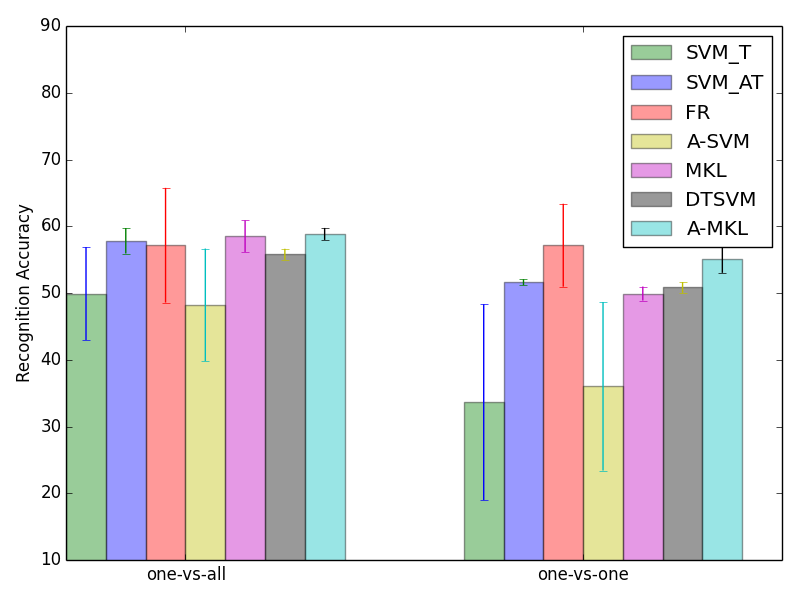
\includegraphics[scale = 0.25]{./onevsone.png}
						\end{figure}

			\column{0.7\textwidth}
				\begin{itemize}
					\item \scriptsize{One-vs-all outperformed one-vs-one}
					\item \scriptsize{Trade-offs between running time and accuracy}
						\begin{enumerate}
							\item \scriptsize{One-vs-all requires more time}
							\item \scriptsize{Domain adaptations require more time}
						\end{enumerate}
				\end{itemize}
		\end{columns}

\end{frame}